\documentclass[12pt]{article}
\usepackage[paper=letterpaper,margin=2cm]{geometry}
\usepackage{amsmath,amssymb,amsfonts}
\usepackage{enumitem}
\usepackage{titling}
\usepackage{multirow}
\usepackage{xcolor}
\usepackage{float}
\usepackage{graphicx}
\usepackage{xcolor}
\definecolor{ISTBlue}{RGB}{0, 139, 255}
\usepackage[colorlinks=true, linkcolor=red]{hyperref}
\usepackage{subcaption} % For subfigures
\usepackage{adjustbox}  % For centering the bottom image
\usepackage{listings}
\usepackage{xcolor} % For setting colors
\usepackage{booktabs} % For better tables
\usepackage{threeparttable} % For table notes

\usepackage{listings}
\usepackage{xcolor}

\definecolor{codegreen}{rgb}{0.0, 0.514, 0.325}      
\definecolor{codegray}{rgb}{0.75, 0.75, 0.75}    
\definecolor{codeblue}{rgb}{0.122, 0.467, 0.706}  
\definecolor{extraLightGray}{rgb}{0.98, 0.98, 0.98}
\definecolor{codepink}{rgb}{0.894, 0.0, 0.443}

\lstdefinestyle{mystyle}{
    backgroundcolor=\color{extraLightGray},
    commentstyle=\color{codegreen},
    keywordstyle=\color{codeblue},
    numberstyle=\tiny\color{codegray},
    stringstyle=\color{codepink},
    basicstyle=\ttfamily\footnotesize,
    breakatwhitespace=false,
    breaklines=true,
    captionpos=b,
    keepspaces=true,
    numbers=left,
    numbersep=5pt,
    showspaces=false,
    showstringspaces=false,
    showtabs=false,
    tabsize=2
}
\lstset{style=mystyle}

\setlength{\droptitle}{-6em}

\begin{document}

\begin{center}
Aprendizagem 2023\\
Homework I --- Group 003\\
(ist1107028, ist1107137)\vskip 1cm
\end{center}

\large{\textbf{Part I}: Pen and paper}\normalsize

\vspace{20pt}
\hspace{-20pt}\textbf{We collected four positive (P) observations,}
\[
\boldsymbol{\{x_1 = (A,0), \quad x_2 = (B,1), \quad x_3 = (A,1), \quad x_4 = (A,0)\}}
\]
\textbf{and four negative (N) observations,}
\[
\boldsymbol{\{x_5 = (B,0), \quad x_6 = (B,0), \quad x_7 = (A,1), \quad x_8 = (B,1)\}}
\]


\hspace{-20pt}\textbf{Consider the problem of classifying observations as positive or negative.}

\vspace{10pt}
\begin{enumerate}[leftmargin=\labelsep]
    \item \textbf{Compute the F1-measure of a $\mathbf{k}$NN with $\mathbf{k =  5}$ and Hamming distance using a
    leave-one-out evaluation schema. Show all calculus.}

    \vspace{10pt}
    We start by calculating Hamming distance between observations. The Hamming distance is the number of positions at which the corresponding symbols are different.\\
    Since we are workin with $k = 5$, we will consider the 5 nearest neighbors of each observation.
    \vspace{10pt}
    
    \begin{table}[H]
        \begin{center}
            \begin{tabular}{c|cccccccc}
            & $x_1$ & $x_2$ & $x_3$ & $x_4$ & $x_5$ & $x_6$ & $x_7$ & $x_8$\\ 
            \hline
                $x_1$ & \-- & 2 & \textbf{\textcolor{codegreen}{1}} & \textbf{\textcolor{codegreen}{0}} & \textbf{\textcolor{codepink}{1}} & \textbf{\textcolor{codepink}{1}} & \textbf{\textcolor{codepink}{1}} & 2 \\ 
                $x_2$ & 2 & \-- & \textbf{\textcolor{codegreen}{1}} & 2 & \textbf{\textcolor{codepink}{1}} & \textbf{\textcolor{codepink}{1}} & \textbf{\textcolor{codepink}{1}} & \textbf{\textcolor{codepink}{0}} \\ 
                $x_3$ & \textbf{\textcolor{codegreen}{1}} & \textbf{\textcolor{codegreen}{1}} & \-- & \textbf{\textcolor{codegreen}{1}} & 2 & 2 & \textbf{\textcolor{codepink}{0}} & \textbf{\textcolor{codepink}{1}} \\ 
                $x_4$ & \textbf{\textcolor{codegreen}{0}} & 2 & \textbf{\textcolor{codegreen}{1}} & \-- & \textbf{\textcolor{codepink}{1}} & \textbf{\textcolor{codepink}{1}} & \textbf{\textcolor{codepink}{1}} & 2 \\ 
                $x_5$ & \textbf{\textcolor{codegreen}{1}} & \textbf{\textcolor{codegreen}{1}} & 2 & \textbf{\textcolor{codegreen}{1}} & \-- & \textbf{\textcolor{codepink}{0}} & 2 & \textbf{\textcolor{codepink}{1}} \\ 
                $x_6$ & \textbf{\textcolor{codegreen}{1}} & \textbf{\textcolor{codegreen}{1}} & 2 & \textbf{\textcolor{codegreen}{1}} & \textbf{\textcolor{codepink}{0}} & \-- & 2 & \textbf{\textcolor{codepink}{1}} \\ 
                $x_7$ & \textbf{\textcolor{codegreen}{1}} & \textbf{\textcolor{codegreen}{1}} & \textbf{\textcolor{codegreen}{0}} & \textbf{\textcolor{codegreen}{1}} & 2 & 2 & \-- & \textbf{\textcolor{codepink}{1}} \\ 
                $x_8$ & 2 & \textbf{\textcolor{codegreen}{0}} & \textbf{\textcolor{codegreen}{1}} & 2 & \textbf{\textcolor{codepink}{1}} & \textbf{\textcolor{codepink}{1}} & \textbf{\textcolor{codepink}{1}} & \-- \\ 
            \end{tabular}
            \caption{Hamming distance between observations, $k=5$}
        \end{center}
    \end{table}

    Now that we have the Hamming distance between all observations, we must identify if the prediction is correct or not. We will consider the majority class of the 5 nearest neighbors for each observation.
    
    \vspace{10pt}
    \underline{Example}: For $x_1$, the 5 nearest neighbors are $x_3$ and $x_4$ (which are positive), $x_5$, $x_6$ and $x_7$ (which are negative). The majority class is negative, therefore the prediction is incorrect.
    
    \newpage
    We apply the same logic for the rest of the classes, ending up with the following table:

    \begin{table}[H]
        \begin{center}
            \begin{threeparttable}
            \begin{tabular}{c|c|c|c|c}
                Observation & True Value & Mode & Prediction & Confusion Matrix Terminology\\
                \hline
                $x_1$ & P &\{$2P, 3N$\}& N & FN\\
                $x_2$ & P &\{$1P, 4N$\}& N & FN\\
                $x_3$ & P &\{$3P, 2N$\}& P & TP\\
                $x_4$ & P &\{$2P, 3N$\}& N & FN\\
                $x_5$ & N &\{$3P, 2N$\}& P & FP\\
                $x_6$ & N &\{$3P, 2N$\}& P & FP\\
                $x_7$ & N &\{$4P, 1N$\}& P & FP\\
                $x_8$ & N &\{$2P, 3N$\}& N & TN\\
            \end{tabular}
            \begin{tablenotes}
                \small
                \item[]
                \item[P - Positive observation; N - Negative observation]  
                \item[TP - True Positive; TN - True Negative; FP - False Positive; FN - False Negative] 
                \item[] 
            \end{tablenotes}
        \end{threeparttable}
            \caption{Predictions for each observation, $k=5$}
        \end{center}
    \end{table}

    With this table, we can know calculate the Precision, Recall and F1-measure using the following formulas:

    \begin{equation}\label{precision}
        \text{Precision} = \frac{\text{True Positives}}{{\text{True Positives} +
        \text{False Positives}}}
    \end{equation}

    \begin{equation}\label{recall}
        \text{Recall} = \frac{\text{True Positives}}{{\text{True Positives} + \text{False Negatives}}}
    \end{equation}

    \begin{equation}\label{f1}
        \text{F1-measure} = 2 \times \frac{{\text{Precision} \times \text{Recall}}}{{\text{Precision} + \text{Recall}}}
    \end{equation}

    \vspace{10pt}
    Replacing the corresponding values in the formulas, we get:

    \vspace{10pt}
    for Precision \eqref{precision} and Recall \eqref{recall}:

    \begin{equation*}
        \text{Precision} = \frac{1}{1 + 3} = 0.25 \quad \quad
        \text{Recall} = \frac{1}{1 + 3} = 0.25
    \end{equation*}

    F1-measure \eqref{f1}:

    \begin{equation*}
        \text{F1-measure} = 2 \times \frac{0.25 \times 0.25}{0.25 + 0.25} = 0.25
    \end{equation*}

    \newpage
    \item \textbf{Propose a new metric (distance) that improves the latter's performance (i.e., the
    F1-measure) by three fold.} 
    
    \vspace{10pt}
    
    To improve the F1-measure, we propose using $k=3$ instead of $k=5$ and to atribute more weight to the difference between letters. 
    
    \vspace{10pt}
    \underline{Example}: When calculating the Hamming distance, if the corresponding $y_1$ values (letters) differ, it counts as 2 instead of 1. For $y_2$, it counts as 1, as in the previous exercise. Below is how we calculated some of the distances to conclude the example:
    \vspace{10pt}
    \begin{align*}
        d(x_1, x_2) &= 2 + 1 = 3 \quad \text{(both } y_1 \text{ and } y_2 \text{ differ)} \\
        d(x_1, x_3) &= 1 \quad \text{(only } y_2 \text{ differs)} \\
        d(x_1, x_5) &= 2 \quad \text{(only } y_1 \text{ differs)}
    \end{align*}
    
    We apply this logic to the rest of the distances, endind up with the next table, where the colored values are the $k=3$ nearest neighbors:
    \vspace{5pt}
    \begin{table}[H]
        \begin{center}
            \begin{tabular}{c|cccccccc}
            & $x_1$ & $x_2$ & $x_3$ & $x_4$ & $x_5$ & $x_6$ & $x_7$ & $x_8$\\ 
            \hline
                $x_1$ & \-- & 3 & \textbf{\textcolor{codegreen}{1}} & \textbf{\textcolor{codegreen}{0}} & 2 & 2 & \textbf{\textcolor{codepink}{1}} & 3\\ 
                $x_2$ & 3 & \-- & 2 & 3 & \textbf{\textcolor{codepink}{1}} & \textbf{\textcolor{codepink}{1}} & 2 & \textbf{\textcolor{codepink}{0}}\\ 
                $x_3$ & \textbf{\textcolor{codegreen}{1}} & 2 & \-- & \textbf{\textcolor{codegreen}{1}} & 3 & 3 & \textbf{\textcolor{codepink}{0}} & 2\\ 
                $x_4$ & \textbf{\textcolor{codegreen}{0}} & 3 & \textbf{\textcolor{codegreen}{1}} & \-- & 2 & 2 & \textbf{\textcolor{codepink}{1}} & 3\\ 
                $x_5$ & 2 & \textbf{\textcolor{codegreen}{1}} & 3 & 2 & \-- & \textbf{\textcolor{codepink}{0}} & 3 & \textbf{\textcolor{codepink}{1}}\\ 
                $x_6$ & 2 & \textbf{\textcolor{codegreen}{1}} & 3 & 2 & \textbf{\textcolor{codepink}{0}} & \-- & 3 & \textbf{\textcolor{codepink}{1}}\\ 
                $x_7$ & \textbf{\textcolor{codegreen}{1}} & 2 & \textbf{\textcolor{codegreen}{0}} & \textbf{\textcolor{codegreen}{1}} & 3 & 3 & \-- & 2\\ 
                $x_8$ & 3 & \textbf{\textcolor{codegreen}{0}} & 2 & 3 & \textbf{\textcolor{codepink}{1}} & \textbf{\textcolor{codepink}{1}} & 2 & \-- \\ 
            \end{tabular}
            \caption{Hamming distance between observations, $k=3$}
        \end{center}
    \end{table}

    Simply by looking at this, we can produce a new prediton table, like in the first exercise:

    \begin{table}[H]
        \begin{center}
            \begin{threeparttable}
            \begin{tabular}{c|c|c|c|c}
                Observation & True Value & Mode & Prediction & Confusion Matrix Terminology\\
                \hline
                $x_1$ & P &\{$2P, 1N$\}& P & TP\\
                $x_2$ & P &\{$0P, 3N$\}& N & FN\\
                $x_3$ & P &\{$2P, 1N$\}& P & TP\\
                $x_4$ & P &\{$2P, 1N$\}& P & TP\\
                $x_5$ & N &\{$1P, 2N$\}& N & TN\\
                $x_6$ & N &\{$1P, 2N$\}& N & TN\\
                $x_7$ & N &\{$3P, 0N$\}& P & FP\\
                $x_8$ & N &\{$1P, 2N$\}& N & TN\\
            \end{tabular}
            \begin{tablenotes}
                \small
                \item[]
                \item[P - Positive observation; N - Negative observation]  
                \item[TP - True Positive; TN - True Negative; FP - False Positive; FN - False Negative] 
                \item[] 
            \end{tablenotes}
        \end{threeparttable}
            \caption{Predictions for each observation, $k=3$}
        \end{center}
    \end{table}

    We can now calculate the Precision \eqref{precision}, Recall \eqref{recall} and F1-measure \eqref{f1}:
    
    \begin{equation*}
        \text{Precision} = \frac{3}{3 + 1} =  0.75 \quad \quad
        \text{Recall} = \frac{3}{3 + 1} = 0.75
    \end{equation*}

    \begin{equation*}
        \text{F1-measure} = 2 \times \frac{0.75 \times 0.75}{0.75 + 0.75} = 0.75 = 3\times0.25
    \end{equation*}


    \vspace{15pt}
    \textbf{An additional positive observation was acquired, $\boldsymbol{x_9 = (B,0)}$, and a third variable $\boldsymbol{y_3}$
    was independently monitored, yielding estimates,}
    \[
    \boldsymbol{y_3|P = \{1.1, 0.8, 0.5, 0.9, 0.8\} \quad and \quad y_3|N = \{1, 0.9, 1.2, 0.9\}}
    \]

    \item \textbf{Considering the nine training observations, learn a Bayesian classifier assuming:
    (i) $\boldsymbol{y_1}$ and $\boldsymbol{y_2}$ are dependent; (ii) {$\boldsymbol{y_1}$, $\boldsymbol{y_2}$} and {$\boldsymbol{y_3}$} variable sets are independent and equally
    important; and (iii) $\boldsymbol{y_3}$ is normally distributed. Show all parameters.}

    \vspace{10pt} 
    With the nine training observations, we can calculate the parameters for the Bayesian classifier.
    We will refer to the outcome, which can be positive or negative, $P$ and $N$ respectively, as `class' or `c'.

    \vspace{10pt} 
    To estimate $P(\text{class} | y_1, y_2, y_3)$, we can use Bayes' theorem:

    \begin{equation}\label{bayes}
        P(\text{class}| y_1, y_2, y_3) = \frac{P(y_1, y_2, y_3 | \text{class}) \times P(\text{class})}{P(y_1, y_2, y_3)}
    \end{equation}

    Since we know $\{y_1, y_2\}$ and $\{y_3\}$ are independent,
    we can rewrite $P(y_1, y_2, y_3)$ as $P(y_1, y_2) \times P(y_3)$.
    Rewriting \eqref{bayes} with this, results in:

    \begin{equation}\label{bayes2}
        P(\text{class}| y_1, y_2, y_3) = \frac{P(y_1, y_2 | \text{class}) \times P(y_3 | \text{class}) \times P(\text{class})}{P(y_1, y_2) \times P(y_3)}
    \end{equation}

    \vspace{10pt}
    We can now begin to compute these parameters.
    \vspace{10pt}
    \begin{equation*}
        \text{Priors:} \qquad
        P(P) = \frac{5}{9} \quad \quad P(N) = 1- P(P) = \frac{4}{9} 
    \end{equation*}

    \vspace{10pt}
    To get the likelihoods, we start by calculating the \textbf{PMFs}:
    \begin{equation*}
        \begin{aligned}
        P((y_1 = A, y_2 = 0)|P) &= \frac{2}{5} \quad P((y_1 = A, y_2 = 0)|N) &= \frac{0}{4}
        \\
        P((y_1 = A, y_2 = 1)|P) &= \frac{1}{5} \quad P((y_1 = A, y_2 = 1)|N) &= \frac{1}{4} 
        \end{aligned}
    \end{equation*}

    \begin{equation*}
        \begin{aligned}
        P((y_1 = B, y_2 = 0)|P) &= \frac{1}{5} \quad P((y_1 = B, y_2 = 0)|N) &= \frac{2}{4}
        \\
        P((y_1 = B, y_2 = 1)|P) &= \frac{1}{5} \quad P((y_1 = B, y_2 = 1)|N) &= \frac{1}{4} 
        \end{aligned}
    \end{equation*}

    \vspace{10pt}
    And now the \textbf{PDFs}:
    \begin{equation*}
        \begin{aligned}
        P((y_1 = A, y_2 = 0)) &= \frac{2}{9} \quad P((y_1 = B, y_2 = 0)) &= \frac{3}{9}
        \\
        P((y_1 = A, y_2 = 1)) &= \frac{2}{9} \quad P((y_1 = B, y_2 = 1)) &= \frac{2}{9} 
        \end{aligned}
    \end{equation*}


    For the $y_3$, we know that it is normally distributed, so we start by calculating the mean and variance for each class:

    \begin{equation*}
            \textbf{\text{mean:}} \quad \mu = \frac{1}{n} \sum_{i=1}^{n} y_i \qquad\qquad\qquad\qquad \textbf{\text{variance:}} \quad \sigma^2 = \frac{1}{n-1} \sum_{i=1}^{n} (y_i - \mu)^2
    \end{equation*}

    \vspace{10pt}
\[
\begin{array}{ll}
    \text{Positive class:} & \\
    \\
    \mu_P = \frac{1.1 + 0.8 + 0.5 + 0.9 + 0.8}{5} = 0.82 \\[10pt]
    \sigma_P^2 = \frac{(1.1 - 0.82)^2 + (0.8 - 0.82)^2 + (0.5 - 0.82)^2 + (0.9 - 0.82)^2 + (0.8 - 0.82)^2}{4} = 0.047 \\[10pt]
    \\
    \text{Negative class:} & \\
    \\
    \mu_N = \frac{1 + 0.9 + 1.2 + 0.9}{4} = 1.0 \\[10pt]
    \sigma_N^2 = \frac{(1 - 1)^2 + (0.9 - 1)^2 + (1.2 - 1)^2 + (0.9 - 1)^2}{3} = 0.02 \\[10pt]
    \\
    \text{Global:} & \\
    \\
    \mu = \frac{1.1 + 0.8 + 0.5 + 0.9 + 0.8 + 1 + 0.9 + 1.2 + 0.9}{9} = 0.9 \\[10pt]
    \sigma^2 = \frac{(1.1 - 0.9)^2 + (0.8 - 0.9)^2 + (0.5 - 0.9)^2 + (0.9 - 0.9)^2 + (0.8 - 0.9)^2 + (1 - 0.9)^2 + (0.9 - 0.9)^2 + (1.2 - 0.9)^2 + (0.9 - 0.9)^2}{8} = 0.04
\end{array}
\]


\vspace{10pt}
With this, we get:
\begin{equation*}
    \mathcal{N}(\mu_{y_3} = 0.82, \sigma_{y_3}^2 = 0.47|P) \quad \mathcal{N}(\mu_{y_3} = 1, \sigma_{y_3}^2 = 0.02|N) \quad \mathcal{N}(\mu_{y_3} = 0.9, \sigma_{y_3}^2 = 0.04)  
\end{equation*}

\vspace{10pt}
    The normal distribution formula is given by:
    \begin{equation}\label{normal-distribution-likelihood}
        \begin{aligned}
            P(y_z|\mu, \sigma^2) = \frac{1}{\sqrt{2\pi \sigma^2}} \exp\left(-\frac{(y_z - \mu)^2}{2\sigma^2}\right)
        \end{aligned}
    \end{equation}

    \newpage
    Having the parameters for the normal distribution, we calculate the likelihoods for $y_3$ as per \eqref{normal-distribution-likelihood}:
    
    \vspace{10pt}
    Positive class:
    \begin{equation*}
        \begin{aligned}
            &P(y_3 = 1.1|\mu_P, \sigma_P^2) = \frac{1}{\sqrt{2\pi \times 0.47}} \exp\left(-\frac{(1.1 - 0.82)^2}{2 \times 0.47}\right) \approx 0.535\\
            &P(y_3 = 0.8|\mu_P, \sigma_P^2) = \frac{1}{\sqrt{2\pi \times 0.47}} \exp\left(-\frac{(0.8 - 0.82)^2}{2 \times 0.47}\right) \approx 0.582\\
            &P(y_3 = 0.5|\mu_P, \sigma_P^2) = \frac{1}{\sqrt{2\pi \times 0.47}} \exp\left(-\frac{(0.5 - 0.82)^2}{2 \times 0.47}\right) \approx 0.522\\
            &P(y_3 = 0.9|\mu_P, \sigma_P^2) = \frac{1}{\sqrt{2\pi \times 0.47}} \exp\left(-\frac{(0.9 - 0.82)^2}{2 \times 0.47}\right) \approx 0.578
        \end{aligned}
    \end{equation*}


    \vspace{10pt}
    Negative class:
    
    \begin{equation*}
        \begin{aligned}
            &P(y_3 = 1|\mu_N, \sigma_N^2) = \frac{1}{\sqrt{2\pi \times 0.02}} \exp\left(-\frac{(1 - 1)^2}{2 \times 0.02}\right) \approx 2.821 \\
            &P(y_3 = 0.9|\mu_N, \sigma_N^2) = \frac{1}{\sqrt{2\pi \times 0.02}} \exp\left(-\frac{(0.9 - 1)^2}{2 \times 0.02}\right) \approx 2.197 \\
            &P(y_3 = 1.2|\mu_N, \sigma_N^2) = \frac{1}{\sqrt{2\pi \times 0.02}} \exp\left(-\frac{(1.2 - 1)^2}{2 \times 0.02}\right) \approx 1.038\\
        \end{aligned}
    \end{equation*}

    Global:
    \begin{equation*}
        \begin{aligned}
            &P(y_3 = 1.1|\mu, \sigma^2) = \frac{1}{\sqrt{2\pi \times 0.04}} \exp\left(-\frac{(1.1 - 0.9)^2}{2 \times 0.04}\right) = 0.5 \\
            &P(y_3 = 0.8|\mu, \sigma^2) = \frac{1}{\sqrt{2\pi \times 0.04}} \exp\left(-\frac{(0.8 - 0.9)^2}{2 \times 0.04}\right) = 0.125\\
            &P(y_3 = 0.5|\mu, \sigma^2) = \frac{1}{\sqrt{2\pi \times 0.04}} \exp\left(-\frac{(0.5 - 0.9)^2}{2 \times 0.04}\right) = 2\\
            &P(y_3 = 0.9|\mu, \sigma^2) = \frac{1}{\sqrt{2\pi \times 0.04}} \exp\left(-\frac{(0.9 - 0.9)^2}{2 \times 0.04}\right) = 0\\
            &P(y_3 = 1.0|\mu, \sigma^2) = \frac{1}{\sqrt{2\pi \times 0.04}} \exp\left(-\frac{(1.0 - 0.9)^2}{2 \times 0.04}\right) = 0.125\\
            &P(y_3 = 1.2|\mu, \sigma^2) = \frac{1}{\sqrt{2\pi \times 0.04}} \exp\left(-\frac{(1.2 - 0.9)^2}{2 \times 0.04}\right) = 1.125
        \end{aligned}
    \end{equation*}

    \vspace{10pt}
    Now we have all the parameters to apply the Bayesian classifier to new observations.

    \vspace{20pt}
    \textbf{Consider now three testing observations,} 
    \begin{equation*}
        {\boldsymbol{\{(A, 1, 0.8), (B, 1, 1), (B, 0, 0.9)\}}}
    \end{equation*}

    \item \textbf{Under a MAP assumption, classify each testing observation showing all your
    calculus.}

    \vspace{10pt}
    MAP (Maximum A Posteriori) is defined as:
    
    \begin{equation}\label{map}
        \begin{aligned}
          \hat{z} & = \underset{c_i}{\text{arg max}} \medspace \left\{P(c_i | x)\right\} \\
                  & = \underset{c_i}{\text{arg max}} \medspace \left\{\frac{P(x | c_i)  \times P(c_i)}{P(x)}\right\} \\
                  & = \underset{c_i}{\text{arg max}} \medspace \left\{P(x | c_i)  \times P(c_i)\right\} \quad \hfill \text{\small{Denominator will be the same for all calculated values.}}
        \end{aligned}
    \end{equation}

    \vspace{10pt}
    To apply this assumption we use the likelihoods and the priors calculated in the lattest exercise.
    We must also calculate the missing values needed - $P(y_3 = 0.8|\mu_N, \sigma_N^2)$ and $P(y_3 = 1|\mu_P, \sigma_P^2)$.

    \begin{equation*}
        \begin{aligned}
            P(y_3 = 0.8|\mu_N, \sigma_N^2) &= \frac{1}{\sqrt{2\pi \times 0.02}} \exp\left(-\frac{(0.8 - 1)^2}{2 \times 0.02}\right) \approx 2.821\\
            P(y_3 = 1|\mu_P, \sigma_P^2) &= \frac{1}{\sqrt{2\pi \times 0.47}} \exp\left(-\frac{(1 - 0.82)^2}{2 \times 0.47}\right) \approx 0.535
        \end{aligned}
    \end{equation*}

    \vspace{10pt}
    With this, we can replace the values in the MAP formula \eqref{map} for each observation:

    \vspace{10pt}
    \fbox{$(A, 1, 0.8)$}
    \begin{equation*}
        \begin{aligned}
        P(y_1 = A, y_2 = 1, y_3 = 0.8 | P) &= P(y_1 = A, y_2 = 1 | \text{P}) \times P(y_3 = 0.8 | \text{P}) \times P(P) \\
        &= \frac{1}{5} \times 0.582 \times \frac{5}{9} \approx 0.065\\
        \\
        P(y_1 = A, y_2 = 1, y_3 = 0.8 | N) &= P(y_1 = A, y_2 = 1 | \text{N}) \times P(y_3 = 0.8 | \text{N}) \times P(N) \\
        &= \frac{1}{4} \times 2.197 \times \frac{4}{9} \approx 0.488\\
        \end{aligned}
    \end{equation*}

    \begin{equation*}
    \begin{aligned}
        \hat{z}_{(A, 1, 0.8)} &= \underset{c \in \{P,N\}}{\text{arg max}} \medspace \left\{P(y_1 = A, y_2 = 1 | c) P(y_3 = 0.8| c) \times P(c)\right\}\\
                    & = \text{arg max} \medspace \left\{P(y_1, y_2 | P) P(y_3| P) \times P(P); P(y_1, y_2 | N) P(y_3| N) \times P(N)\right\} \\
                    & = N
    \end{aligned}
    \end{equation*}

    \fbox{$(B, 1, 1)$}
    \begin{equation*}
        \begin{aligned}
        P(y_1 = B, y_2 = 1, y_3 = 1 | P) &= P(y_1 = B, y_2 = 1 | \text{P}) \times P(y_3 = 1 | \text{P}) \times P(P) \\
        &= \frac{1}{5} \times 2.821 \times \frac{5}{9} \approx 0.313\\
        \\
        P(y_1 = B, y_2 = 1, y_3 = 1 | N) &= P(y_1 = B, y_2 = 1 | \text{N}) \times P(y_3 = 1 | \text{N}) \times P(N) \\
        &= \frac{1}{4} \times 0.535 \times \frac{4}{9} \approx 0.059\\
        \end{aligned}
    \end{equation*}
    
    \begin{equation*}
        \begin{aligned}
            \hat{z}_{(B, 1, 1)} &= \underset{c \in \{P,N\}}{\text{arg max}} \medspace \left\{P(y_1 = B, y_2 = 1 | c) P(y_3 = 1| c) \times P(c)\right\}\\
                          & = \text{arg max} \medspace \left\{P(y_1, y_2 | P) P(y_3| P) \times P(P); P(y_1, y_2 | N) P(y_3| N) \times P(N)\right\} \\
                          & = P
        \end{aligned}
    \end{equation*}

    \fbox{$(B, 0, 0.9)$} 
    \begin{equation*}
        \begin{aligned}
        P(y_1 = B, y_2 = 0, y_3 = 0.9 | P) &= P(y_1 = B, y_2 = 0 | \text{P}) \times P(y_3 = 0.9 | \text{P}) \times P(P) \\
        &= \frac{1}{5} \times 0.578 \times \frac{5}{9} \approx 0.064\\
        \\
        P(y_1 = B, y_2 = 0, y_3 = 0.9 | N) &= P(y_1 = B, y_2 = 0 | \text{N}) \times P(y_3 = 0.9 | \text{N}) \times P(N) \\
        &= \frac{2}{4} \times 2.197 \times \frac{4}{9} \approx 0.488\\
        \end{aligned}
    \end{equation*}

    \begin{equation*}
        \begin{aligned}
            \hat{z}_{(B, 0, 0.9)} &= \underset{c \in \{P,N\}}{\text{arg max}} \medspace \left\{P(y_1 = B, y_2 = 0 | c) P(y_3 = 0.9| c) \times P(c)\right\}\\
                          & = \text{arg max} \medspace \left\{P(y_1, y_2 | P) P(y_3| P) \times P(P); P(y_1, y_2 | N) P(y_3| N) \times P(N)\right\} \\
                          & = N 
        \end{aligned}
    \end{equation*}

    \vspace{10pt}
    Therefore, the predictions for each observation are $N$, $P$ and $N$ respectively.

    \vspace{10pt}

    \textbf{At last, consider only the following sentences and their respective connotations,}
    \[
    \boldsymbol{\{("Amazing\; run", P), ("I\; like\; it", P), ("Too\; tired", N), ("Bad\; run", N)\}}
    \]

    \item \textbf{Using a naïve Bayes under a ML assumption, classify the new sentence
    "I like to run". For the likelihoods calculation consider the following formula,}

    \begin{equation*}
        \boldsymbol{P(T_i|c) = \frac{freq(t_i) + 1}{N_c + V}}
    \end{equation*}

    \textbf{where $\mathbf{t_i}$ represents a certain term $\mathbf{i}$, $\mathbf{V}$ the number of unique terms in the vocabulary, and
    $\mathbf{N_c}$ the total number of terms in class $\mathbf{c}$. Show all calculus.}

    
    \vspace{10pt}
    \begin{equation*}
        \begin{aligned}
            \text{Vocabulary:} & \quad \{amazing, run, I, like, it, to, tired, bad\} & Total = 8\\
            \text{Positive class:} & \quad \{amazing, run, I, like, it\} &\qquad N_P = 5\\
            \text{Negative class:} & \quad \{to, tired, bad, run\} &\qquad N_P = 4\\
        \end{aligned}
    \end{equation*}

    \vspace{10pt}
    Now we calculate the likelihoods with the given expression:

    \begin{equation*}
        \begin{aligned}
            P(\text{I}|P) &= \frac{freq(I) + 1}{5+8} = \frac{1+1}{13} \approx 0.154 \qquad P(\text{I}|N) = \frac{freq(I) + 1}{4+8} = \frac{0+1}{12} \approx 0.083\\
            \\
            P(\text{Like}|P) &= \frac{freq(Like) + 1}{5+8} = \frac{1+1}{13} \approx 0.154  \quad P(\text{Like}|N) = \frac{freq(Like) + 1}{4+8} = \frac{0+1}{12} \approx 0.083\\
            \\
            P(\text{to}|P) &= \frac{freq(to) + 1}{5+8} = \frac{0+1}{13} \approx 0.077 \qquad P(\text{to}|N) = \frac{freq(to) + 1}{4+8} = \frac{0+1}{12} \approx 0.083\\
            \\
            P(\text{run}|P) &= \frac{freq(run) + 1}{5+8} = \frac{1+1}{13} \approx 0.154 \qquad P(\text{run}|N) = \frac{freq(run) + 1}{4+8} = \frac{1+1}{12} \approx 0.167\\
        \end{aligned}
    \end{equation*}

    \vspace{10pt}
    ML assumption can be defined as follows:

    \begin{equation}\label{ml}
        \begin{aligned}
            \hat{z} & = \underset{c_i}{\text{arg max}} \medspace \left\{P(c_i | x)\right\} \\
                    & = \underset{c_i}{\text{arg max}} \medspace \left\{\frac{P(x | c_i)  \times P(c_i)}{P(x)}\right\} \\
                    & = \underset{c_i}{\text{arg max}} \medspace \left\{P(x | c_i)\right\} \\
        \end{aligned}
    \end{equation}
   
    We must caclulate the probabilities for the sentence "I like to run" for both classes.

    \begin{equation*}
        \begin{aligned}
            P(\text{"I like to run"}|P) &= P(I|P) \cdot P(\text{like}|P) \cdot P(\text{to}|P) \cdot P(\text{run}|P) \\
            &= 0.154 \times 0.154 \times 0.077 \times 0.154 \approx 0.00028\\
            \\
            P(\text{"I like to run"}|N) &= P(I|N) \cdot P(\text{like}|N) \cdot P(\text{to}|N) \cdot P(\text{run}|N) \\
            &= 0.083 \times 0.083 \times 0.083 \times 0.167 \approx 0.000095\\
        \end{aligned}
    \end{equation*}
    \vspace{10pt}
    Replacing the values in \eqref{ml}, we get:
    \begin{equation*}
        \begin{aligned}
            \hat{z}_{\text{"I like to run"}} &= \underset{c \in \{P,N\}}{\text{arg max}} \left\{P(I | c) \cdot P(\text{like}| c) \cdot P(\text{to}|c) \cdot P(\text{run}|c)\right\}\\
            &= \text{arg max} \left\{0.00028, 0.000095\right\} = P
        \end{aligned}
    \end{equation*}    

    \end{enumerate}

    \newpage

    \large{\textbf{Part II}: Programming}\normalsize

    \vspace{20pt}
    \textbf{Consider the heart-disease.csv dataset available at the course webpage's homework tab. Using sklearn, apply a 5-fold stratified cross-validation with shuffling (random\_state = 0) for the assessment of predictive models along this section.}

    \vspace{10pt}
    \textbf{(1) Compare the performance of a $\mathbf{kNN}$ with $\mathbf{k=5}$ and a Naive Bayes with Gaussian assumption (consider all remaining parameters as default):}

    \vspace{10pt}
    \textbf{a. Plot two boxplots with the fold accuracies for each classifier. Is there one
    more stable than the other regarding performance? Why do you think that is the
    case? Explain.}

    \vspace{20pt}
    \lstinputlisting[language=Python]{./Part II/1_a.py}

        \begin{figure}[H]
            \centering
            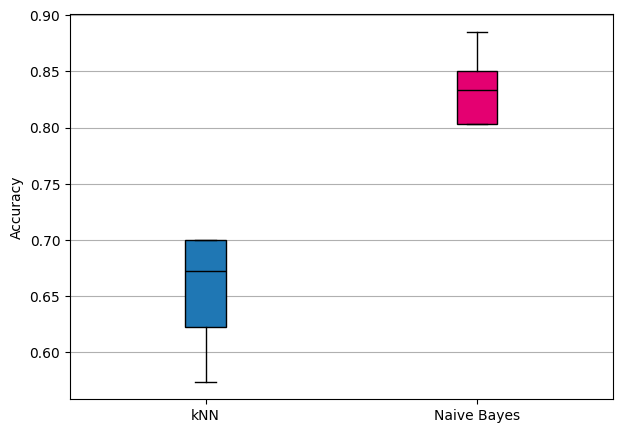
\includegraphics[width=12cm]{./Part II/1_a.png}
            \caption{Boxplot of the fold accuracies for each classifier}
        \end{figure}

    \vspace{20pt}

    None have the models contain outliers, but, regarding performance, the naïve Bayes model apears to be more stable. We make this statment becouse, as we can see in the graph, its boxplot is narrower, which means that its accuracy values are clustered closely around the median, and it also has shorter whiskers, indicating more consistence perform and, therefore, better stability.
    Possible reasons that explain why kNN performs better compared to the naïve Bayes model are:
    \begin{itemize}
        \item kNN is able to handle variable dependencies (naïve Bayes assumes that the features are conditionally independent given the class) and variables that are not normally distributed (naïve Bayes with Gaussian assumption assumes all variables follow this specific distribution).
        \item Naive Bayes can struggle to estimate probabilities accurately when there are too few data points, which may result in incorrect or even zero probabilities. Additionally, if the class distribution is imbalanced, it can lead to biased predictions because the prior probabilities used in the model's calculations may be skewed.
    \end{itemize}


    \vspace{20pt}
    \textbf{b. Report the accuracy of both models, this time scaling the data with a
    Min-Max scaler before training the models. Explain the impact that this
    preprocessing step has on the performance of each model, providing an
    explanation for the results.}

    \vspace{20pt}
    \lstinputlisting[language=Python]{./Part II/1_b.py}

    \begin{figure}[H]
        \centering
        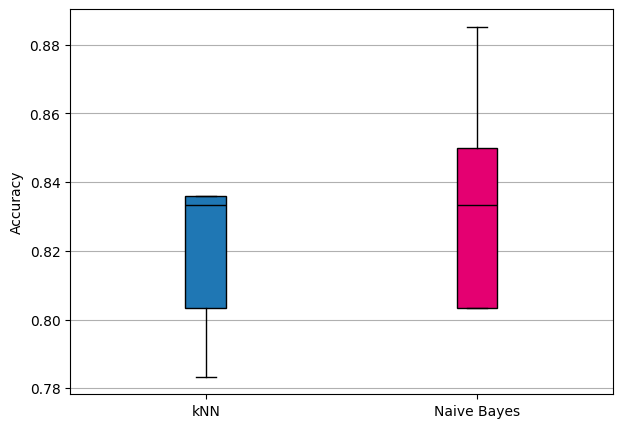
\includegraphics[width=12cm]{./Part II/1_b.png}
        \caption{Accuracy of both models with Min-Max scaling}
    \end{figure}

    \vspace{20pt}
    This pre-processing step worsens the performances of both models. The possible reasons for this outcome is that scaling might make irrelevant features more prominent, reducing both models' effectiveness.

    \begin{itemize}
        \item For kNN, the Min-Max scaler alters the distances that the model relies on, which changes the neighbors that are considered "close", leading to incorret classifications.
        Scaling makes all feature ranges the same, which can decrease the impact of features that were originally more significant, leading to worse performance.
        \item For naïve Bayes, Min-Max scaling can distort the features, making them not normally distributed, which leads to inaccurate probability estimates.
    \end{itemize}

    \vspace{10pt}
    \textbf{c. Using scipy, test the hypothesis "the $\mathbf{kNN}$ model is statistically superior to naive Bayes regarding accuracy", asserting whether it is true.}

    \vspace{10pt}
    Since the p-value ($\text{p-value} = 0.83$), is greater than the usual significance levels, (e.g., $\alpha = 0.05$), we cannot reject the null hypothesis, thus we can't afirm that the kNN model is statistically superior to naïve Bayes regarding accuracy.
    In order to be able to make a correct statement about this hypothesis, it would be necessary to obtain more statistical tests.

    \vspace{20pt}
    \textbf{(2) a 80-20 train-test split, vary the number of neighbors of a $\mathbf{kNN}$ classifier using $\mathbf{k=\{1, 5, 10, 20, 30\}}$. Additionally, for each $k$, train one classifier using uniform weights and distance weights.}

    \vspace{10pt}
    \textbf{a. Plot the train and test accuracy for each model}

    \vspace{20pt}
    \lstinputlisting[language=Python]{./Part II/2_a.py}

    \begin{figure}[H]
        \centering
        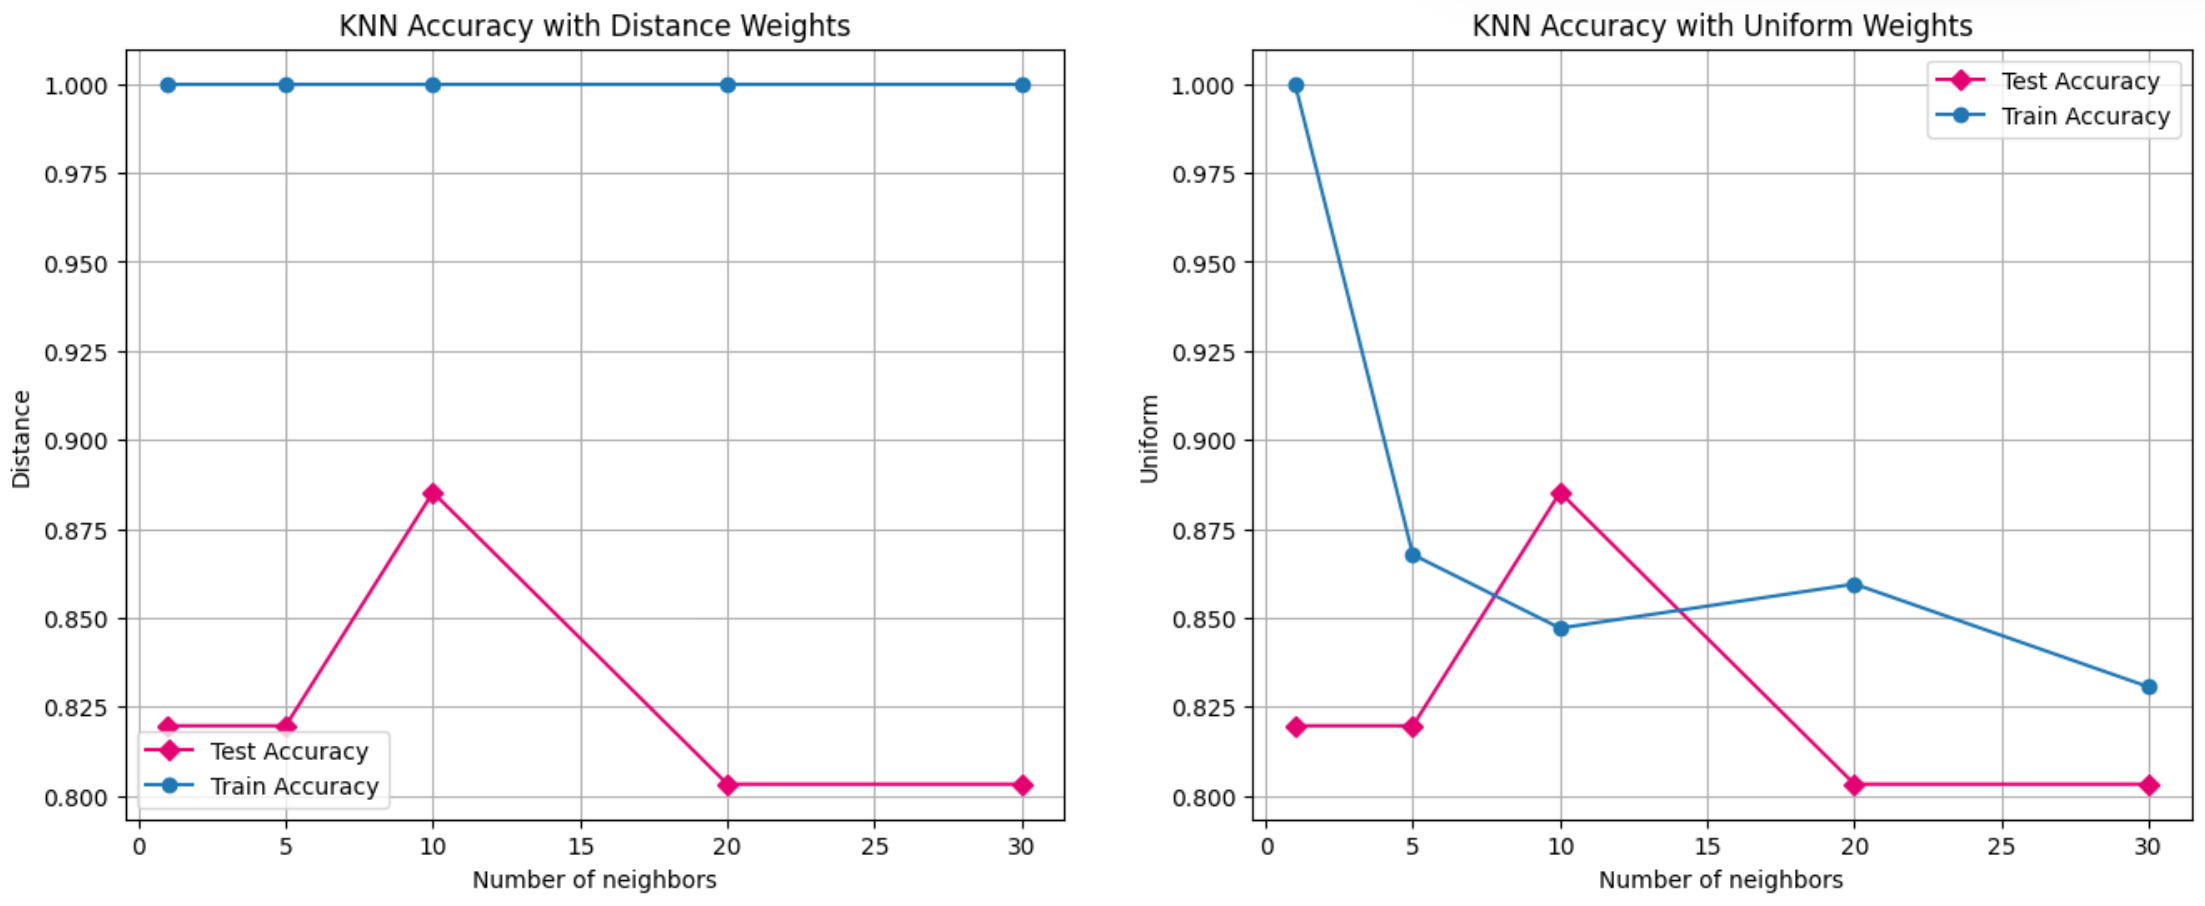
\includegraphics[width=12cm]{./Part II/2_a.png}
        \caption{Train and test accuracy for each model}
    \end{figure}

    \vspace{20pt}
    \textbf{b. Explain the impact of increasing the neighbors on the generalization ability of the models.}

    \vspace{10pt}
    As the number of neighbors (k) increases, both models experience a shift in generalization ability. With uniform weights, as k increases, the model smooths its decision boundaries, reducing training accuracy and improving generalization until it peaks at k = 10. Beyond that, both training and test accuracy drop, indicating underfitting.
    In the case of distance weights, the model maintains perfect training accuracy across all k, suggesting overfitting persists due to the emphasis on closer neighbors. However, the test accuracy also peaks at $k = 10$, similar to uniform weights. After this, increasing k causes underfitting in both models, as they fail to generalize well to the test data. In short, k = 10 is optimal, with larger k values leading to a loss of model generalization in both cases.


    \vspace{20pt}
    \textbf{(3) Considering the unique properties of the heart-disease.csv dataset, identify two
    possible difficulties of the naïve Bayes model used in the previous exercises when learning
    from the given dataset.}

    \vspace{10pt}
    Two possible difficulties are:

    \begin{itemize}
        \item Naïve Bayes assumes class conditional independence, which can lead to a loss of accuracy and the unrealistic assumption of independence between features, such as age and cholesterol. The presence of a heart disease may be more strongly correlated with certain features than others, which would not be captured by the model.
        \item The model assumes that all features follow a specific distribution, which may not accurately reflect the dataset's true distribution, which would lead to inaccurate probability estimates and incorrect classifications.
    \end{itemize}

\end{document}
